\documentclass{article}
\usepackage[utf8]{inputenc}
% important for graphicx
\usepackage{graphicx}
\graphicspath{ {img/} }
\usepackage{float}
\usepackage{enumitem}
\usepackage[]{algorithm2e}
% background color for definitions
\usepackage[most]{tcolorbox}
\tcbset{
    frame code={}
    center title,
    left=0pt,
    right=0pt,
    top=0pt,
    bottom=0pt,
    colback=blue!6!white,
    colframe=white,
    width=\dimexpr\textwidth\relax,
    enlarge left by=0mm,
    boxsep=10pt,
    arc=0pt,outer arc=0pt,
}


\begin{document}

\title{Image Processing \\
Homework 1}
\author{Aadil Anil Kumar \\
Otmane Sabir
}
\date{10/2/2020}
\maketitle
\vspace{10mm}
\begin{center}
\section*{Introduction}
\large
The first homework assignment required us to implement two morphological operations - opening \& closing - while following certain guidelines which could be summarized to the following list: 
\vspace{7mm}
\begin{enumerate}
    \item Writing a command line program that performs either an erosion or a dilation of a given two-dimensional gray-scale image 'f' with respect to a (symmetric, odd-sized) structuring element.
    \item Output a single CSV file for the eroded/dilated image in the same format and same definition and value domains as the input image 'f'.
    \item Do meaningful (motivated from a real-world perspective) openings and closings on at least three photographs or 2D images of our choice. The three chosen problems should be very different in nature and write in the a description of each of the three problems, purpose of the operations to be applied, choice of structuring elements, and provide the output as graphics file.
\end{enumerate}
\end{center}
\newpage

\tableofcontents

\newpage

\section{Dilation \& Erosion}
The realm of morphological operations is based off of certain primitive operations such as dilation and erosion. In the simplest of definitions, dilation adds pixels to the boundaries of objects in an image, while erosion removes pixels on object boundaries. The structuring element defines the range and size of pixels which were added/removed. 
\newline
As we have previously seen in the lecture we can define grayscale erosion with the following : \newline
\begin{tcolorbox}
Denoting an image by $f(x)$ and the grayscale structuring element by $b(x)$, where B is the space that $b(x)$ is defined, the grayscale erosion of $f$ by $b$ is given by :
\newline
\begin{center}
$(f \ominus b)(x) = \inf\limits_{y \in B}[f(x + y) - b[y)]$.
\end{center}

where $inf$ denotes the infimum.
\end{tcolorbox}
While dilation is defined by :
\newline
\begin{tcolorbox}
Denoting an image by $f(x)$ and the grayscale structuring element by $b(x)$, where B is the space that $b(x)$ is defined, the grayscale erosion of $f$ by $b$ is given by :
\newline
\begin{center}
$(f \ominus b)(x) = \sup\limits_{y \in B}[f(x + y) - b[y)]$.
\end{center}

where $sup$ denotes the supermum.
\end{tcolorbox}
\section{Implementation}

We can see by examining the expressions for the morphological dilation or erosion that we're required to get the minimum/maximum of a pixel within the structuring element. Therefore, we first started by implement 2 function $minVal \& maxVal$ which set the value of the output pixel is the max/min value of the pixels that are in neighborhood the size of the SE within the input image. The following algorithm $maxVal$ gets the maximum value which we'll use for the dilation. This function receives the matrix, the current x and y indices we're checking, the maximum value present in this matrix and the structuring element. The $minVal$ algorithm follows the same logic except we check if the current value is less than the stored one and not bigger and also gets the largest value present in the matrix instead of the smallest. 

\subsection{Dilation algorithm}

\begin{algorithm}[H]
 \KwData{matrix, se, maxi val, a, b}
 \KwResult{the min value of the pixels that are in neighborhood the size of the SE}
 initialization\;
 \State $rows\gets$ number of rows in se\;
 \State $cols \gets$ number of cols in se\;
 \State $mRows \gets$ number of rows in matrix\;
 \State $mCols \gets$ number of cols in matrix\;
 \While{$i\leq rows-1$}{
    \While{$j\leq cols-1$}{
        \eIf{$se[i][j] == 1$}{
            \eIf{$0 \geq b \leq mRows - 1$}{
                \eIf{$matrix[a][b]\geq maxi$}
                    {$maxi = matrix[a][b]$\;}
                    {continue\;}
                    $b++$
            }
                {do nothing\;}
        }
            {break\;}
    }
    \eIf{$0 \geq a \leq mCols - 1$}{
    $a++$\;
    reset b to initial value\;
    }{
    }
 }
\Return{maxi}
\newline
\caption{Algorithm to find maximum for dilation}
\end{algorithm}
\vspace{3mm}
After we're able to extract the maximum value within the neighboring area of a pixel then we can write our dilation algorithm. Again, the erosion is the same except we use the $minVal$ algorithm.

\begin{algorithm}[H]
 \KwData{matrix, structuring element}
 \KwResult{the dilated matrix}
 initialization\;
 \State $ans\gets$ empty 2D array of identical size to matrix\;
 \State $mRows \gets$ number of rows in matrix\;
 \State $mCols \gets$ number of cols in matrix\;
 \While{$i\leq mRows$}{
    \While{$j\leq mCols$}{
        \State $ans[i][j] \gets maxVal(matrix, se, i, j)$\;
        increment j\;
    }
    increment i\;
 }
 \caption{Dilation algorithm}
\end{algorithm}
\vspace{8mm}
\subsection{Erosion algorithm}


\begin{algorithm}[H]
 \KwData{matrix, se, min val, a, b}
 \KwResult{the min value of the pixels that are in neighborhood the size of the SE}
 initialization\;
 \State $rows\gets$ number of rows in se\;
 \State $cols \gets$ number of cols in se\;
 \State $mRows \gets$ number of rows in matrix\;
 \State $mCols \gets$ number of cols in matrix\;
 \While{$i\leq rows-1$}{
    \While{$j\leq cols-1$}{
        \eIf{$se[i][j] == 1$}{
            \eIf{$0 \geq b \leq mRows - 1$}{
                \eIf{$matrix[a][b]\leq min$}
                    {$min = matrix[a][b]$\;}
                    {continue\;}
                    $b++$
            }
                {do nothing\;}
        }
            {break\;}
    }
    \eIf{$0 \geq a \leq mCols - 1$}{
    $a++$\;
    reset b to initial value\;
    }{
    }
 }
\Return{maxi}
\newline
\caption{Algorithm to find minimum for erosion}
\end{algorithm}
\vspace{3mm}

\begin{algorithm}[H]
 \KwData{matrix, structuring element}
 \KwResult{the dilated matrix}
 initialization\;
 \State $ans\gets$ empty 2D array of identical size to matrix\;
 \State $mRows \gets$ number of rows in matrix\;
 \State $mCols \gets$ number of cols in matrix\;
 \While{$i\leq mRows$}{
    \While{$j\leq mCols$}{
        \State $ans[i][j] \gets minVal(matrix, se, i, j)$
        increment j\;
    }
    increment i\;
 }
 \caption{Erosion algorithm}
\end{algorithm}

\section{Experiments & Results}
\subsection{Erosion using symmetric vs asymmetric SE}
\vspace{8mm}
\begin{figure}[ht!] 
  \label{ fig7} 
  \begin{minipage}[b]{0.5\linewidth}
    \centering
    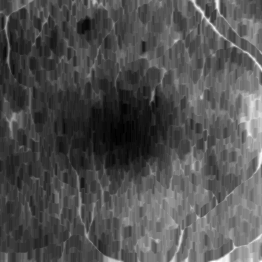
\includegraphics[width=.95\linewidth]{eroSym.png} 
    \caption{Erosion with Symmetric SE} 
    \vspace{4ex}
  \end{minipage}%%
  \begin{minipage}[b]{0.5\linewidth}
    \centering
    \includegraphics[width=.95\linewidth]{eroAsym.png} 
    \caption{Erosion with Asymmetric SE} 
    \vspace{4ex}
  \end{minipage} 
 \end{figure}
\begin{flushleft}
Border effects tend to occur when using an asymmetric SE that does not fit the definition domain of the image set.
As expected the chosen border handling method does introduce artifacts to the image.\\ \\
A possible explanation for this could be the fact that the definition domain of the image set decreases when doing the operation due to image borders not being handled correctly.\\ \\
If you were to observe and compare Figure 1 and 2 closely you can see that the bottom border of Figure 2 contains a row of white space. This is evident when viewing the image with a black background. The effects were more pronounced when doing a comparison of the closing operation, as shown in figure 3 and 4.
\end{flushleft}
\begin{figure}[ht!]
  \begin{minipage}[b]{0.5\linewidth}
    \centering
    
\includegraphics[width=.95\linewidth]{closSym.jpg} 
    \caption{Closing with Symmetric SE} 
    \vspace{4ex}
  \end{minipage}%% 
  \begin{minipage}[b]{0.5\linewidth}
    \centering
    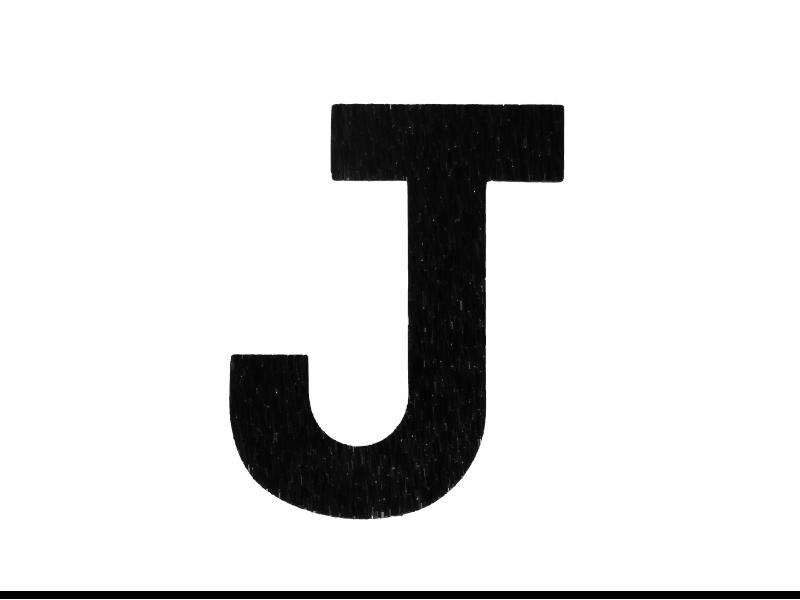
\includegraphics[width=.95\linewidth]{closAsym.jpg} 
    \caption{Closing with Asymmetric SE} 
    \vspace{4ex}
  \end{minipage} 
\end{figure}
\vspace{5mm}

\subsection{Improving the clarity of handwritten digits}
\vspace{6mm}
\begin{figure}[ht!]
  \begin{minipage}[b]{0.5\linewidth}
    \centering
    
\includegraphics[width=.95\linewidth]{six.png} 
    \caption{Original Image 
    \small(602\times599)} 
    \vspace{4ex}
  \end{minipage}%% 
  \begin{minipage}[b]{0.5\linewidth}
    \centering
    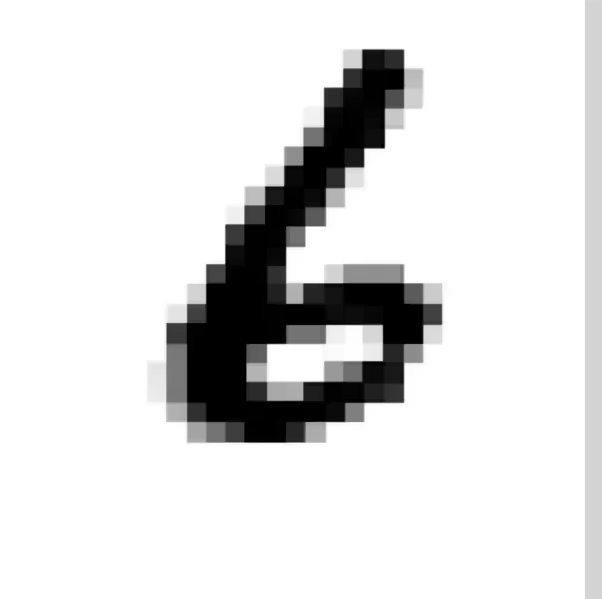
\includegraphics[width=.95\linewidth]{dilated_six.png} 
    \caption{Dilated Six Digit} 
    \vspace{4ex}
  \end{minipage} 
\end{figure}
\begin{flushleft}
As visible in Figure 5, the six is not very well defined and specifically the white circle in the middle. This situation could raise problems with the classification of handwritten digits. Therefore, we dilate the image with a structuring element that is a square of size 15 (SE10.txt) in order to obtain we get a sharper six. We chose this structuring element because we noticed that the six was formed using square blots. We decided to use a larger structuring element because the image is very pixelated and we wanted to obtain a clear circle in the center of the six.
A possible use case for this would be feature extraction. A classification algorithm could more efficiently extract features that maps the digit as a six.
\end{flushleft}
\vspace{8mm}
% ------------
% EXPIREMENT 3
% ------------
\subsection{Cell segmentation}
\vspace{4mm}
\begin{flushleft}
For these operations we used a parallelogram structuring element (SE11.txt). We chose this shape for this image as there are a lot of circular structures that we wanted to highlight. There is a lot more contrast in the images that had the operations done on them; helping clearly segment each cellular structure.
\newline
The dilated image has the clearest segmentation between structures. However, the opened image also shows clear segmentation while not having as jarring of a contrast. This helps us achieve clear segmentation of cells in order to assist with counting.
\end{flushleft}
\begin{figure}[ht!]
    \centering
    \includegraphics[width=7cm]{nuclei.png}
    \caption{Original image (1344\times1024)}
    \label{fig:erosionSym}
\end{figure}
\begin{figure}[ht] 
  \label{ fig7} 
  \begin{minipage}[b]{0.5\linewidth}
    \centering
    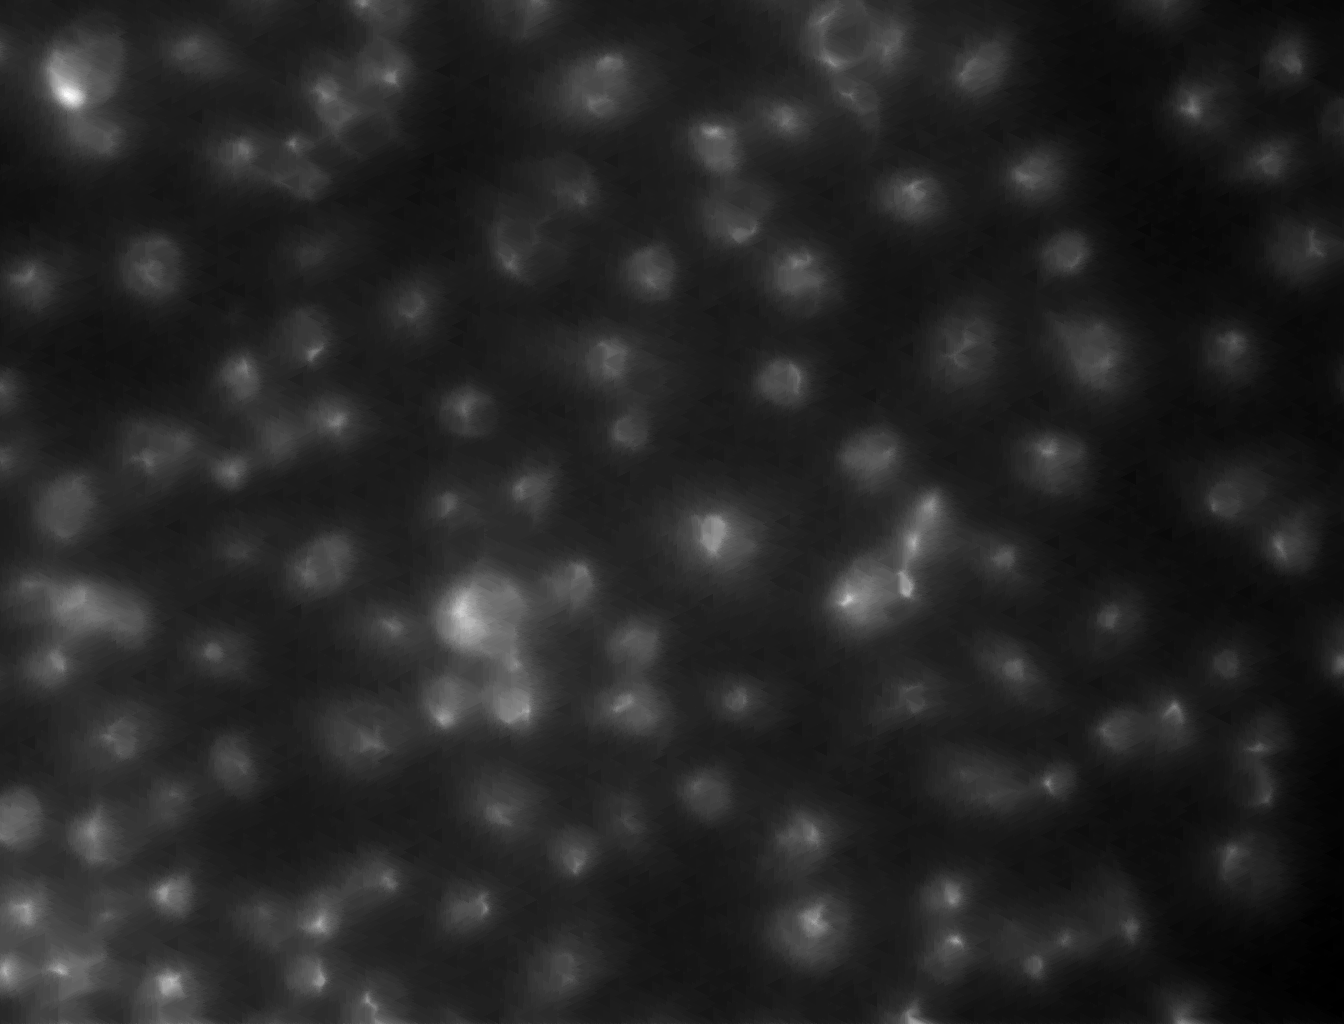
\includegraphics[width=.95\linewidth]{nuclei_erosion.png} 
    \caption{Erosion} 
    \vspace{4ex}
  \end{minipage}%%
  \begin{minipage}[b]{0.5\linewidth}
    \centering
    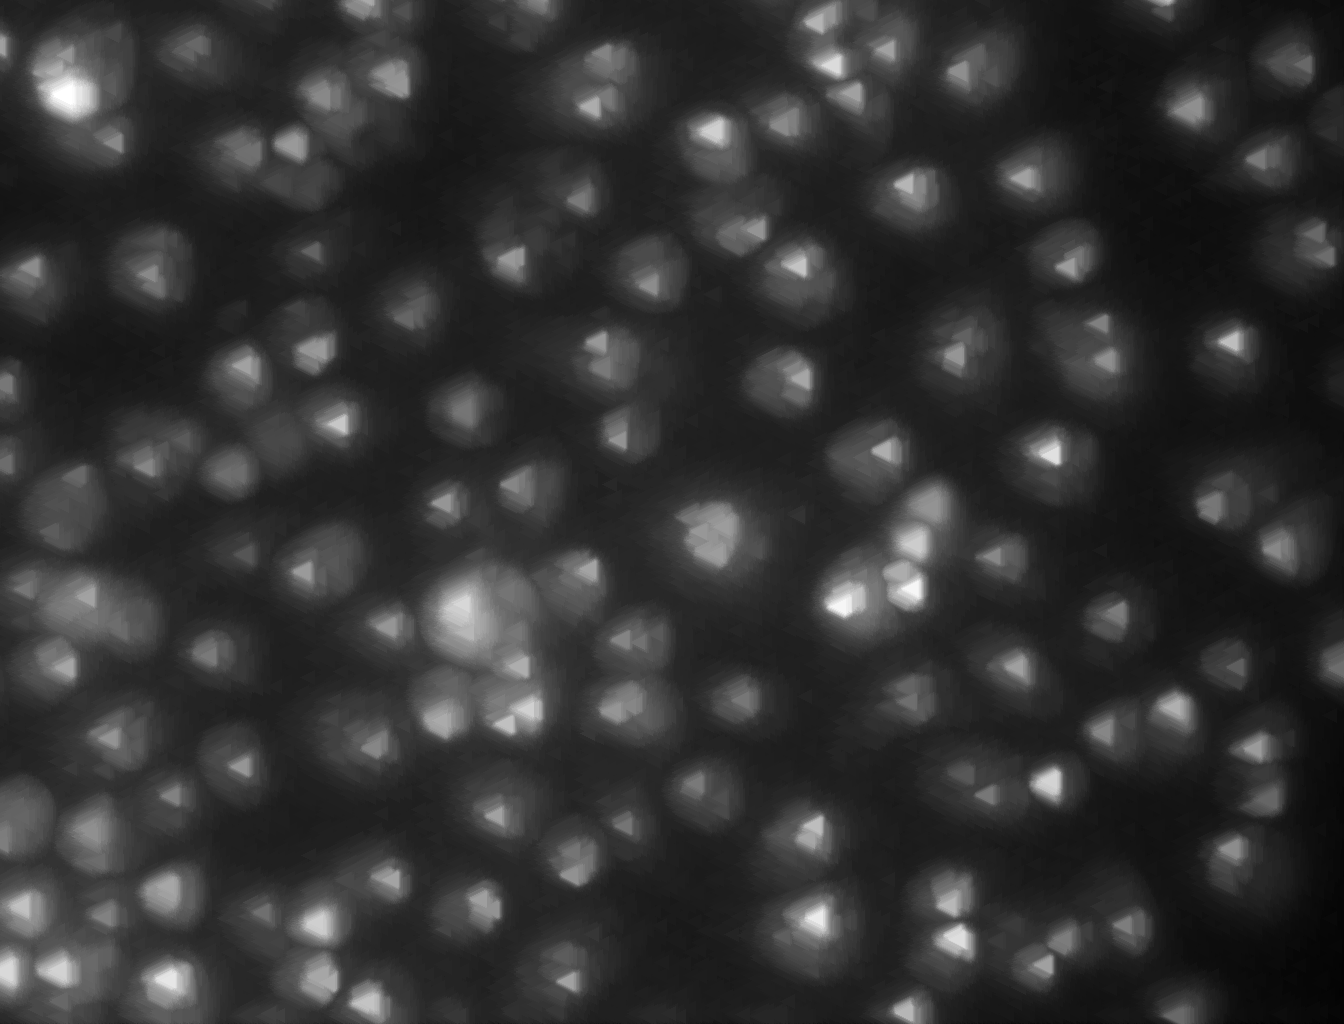
\includegraphics[width=.95\linewidth]{nuclei_dilation.png} 
    \caption{Dilation} 
    \vspace{4ex}
  \end{minipage} 
  \begin{minipage}[b]{0.5\linewidth}
    \centering
    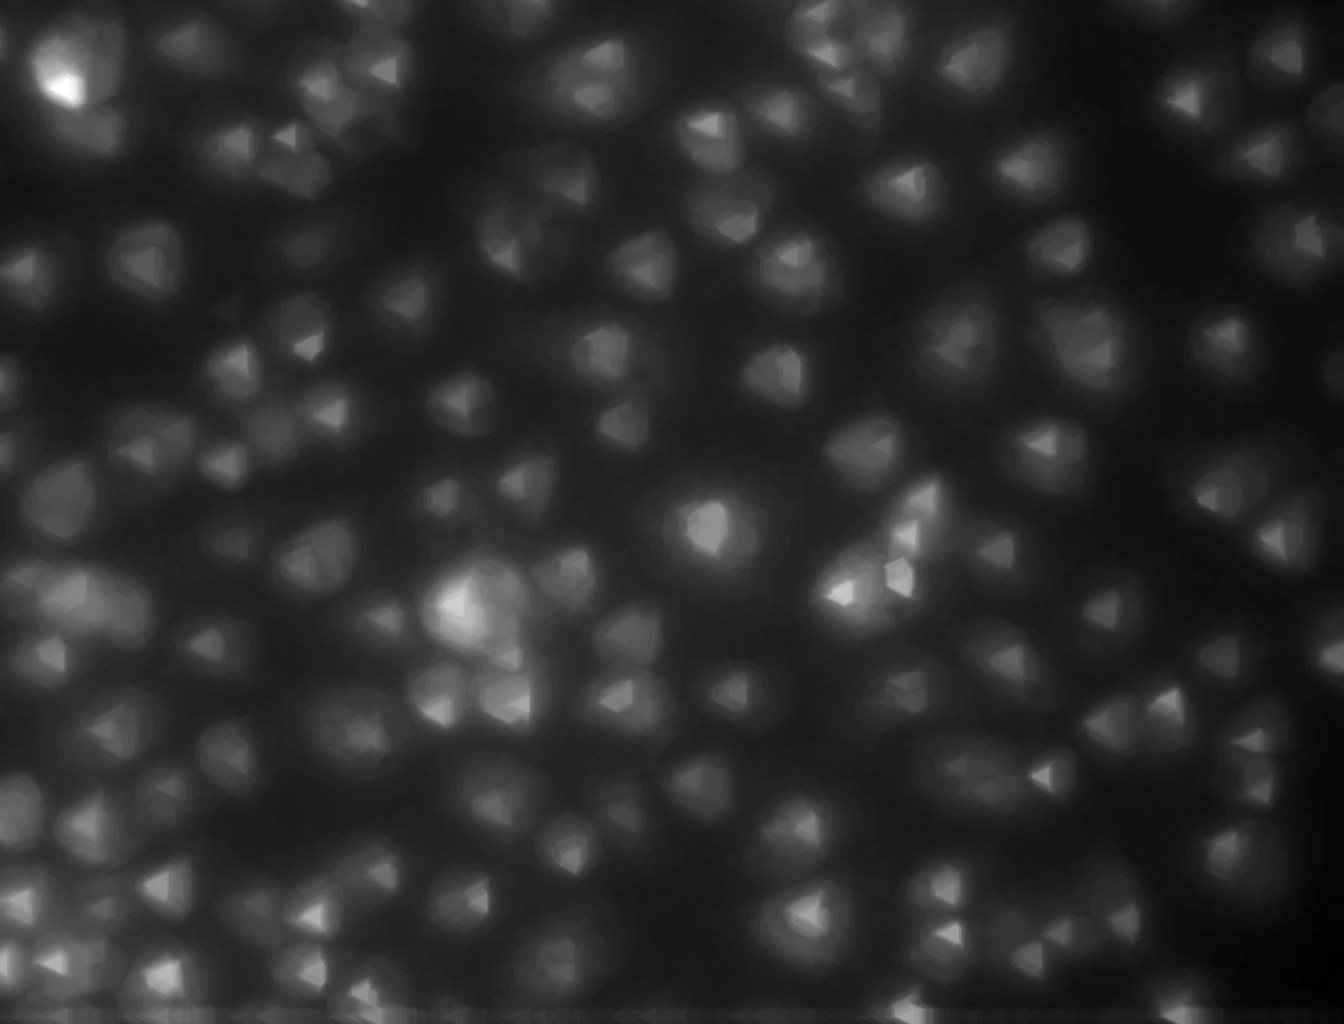
\includegraphics[width=.95\linewidth]{opening.png} 
    \caption{Opening} 
    \vspace{4ex}
  \end{minipage}%% 
  \begin{minipage}[b]{0.5\linewidth}
    \centering
    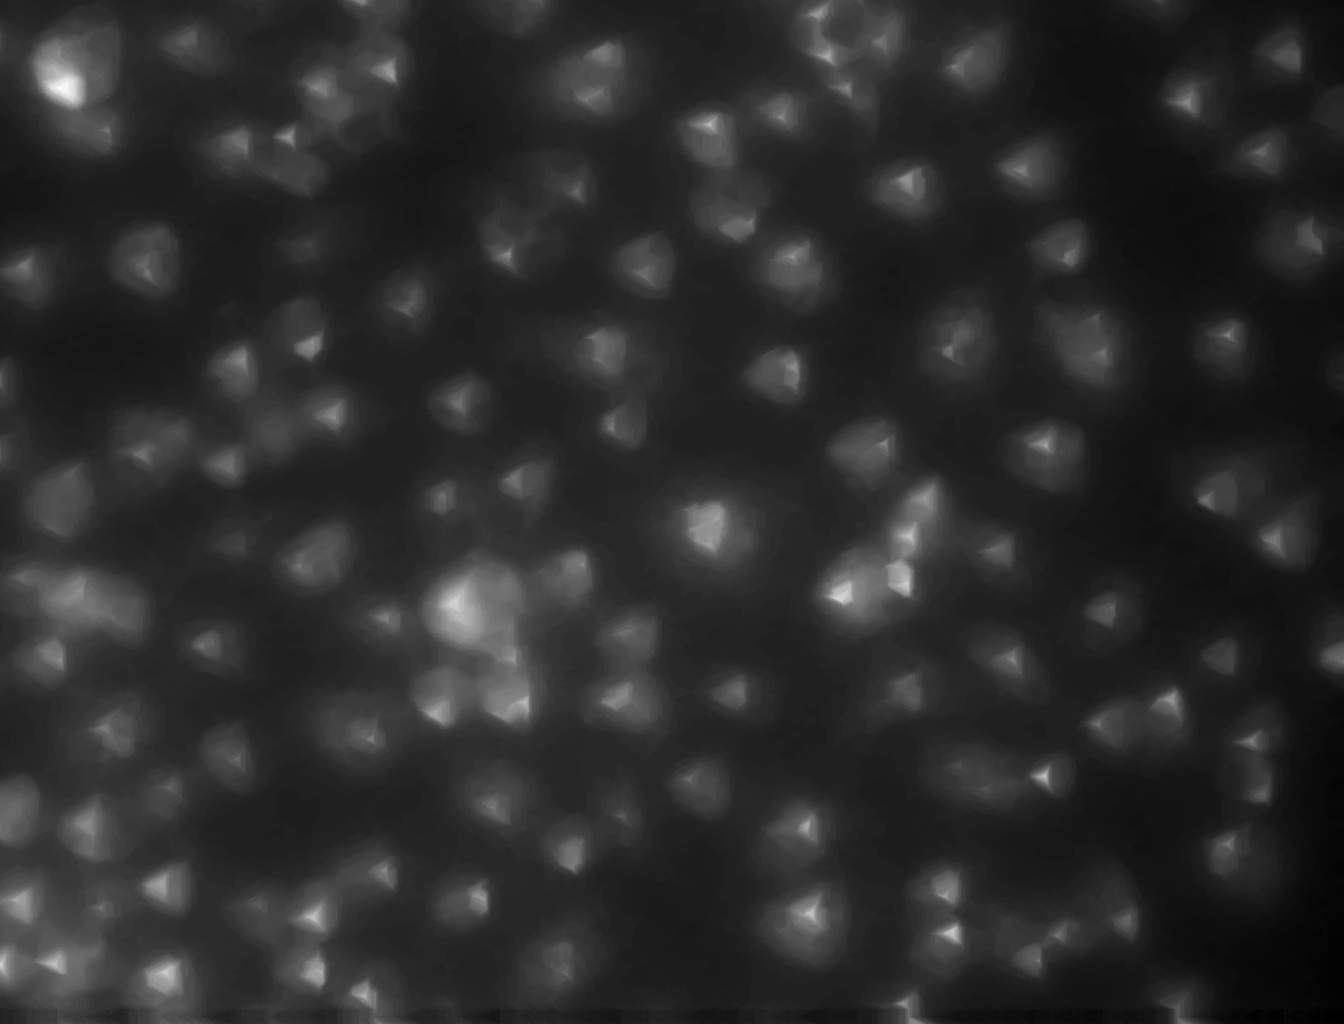
\includegraphics[width=.95\linewidth]{nuclei_closing.png} 
    \caption{Closing} 
    \vspace{4ex}
  \end{minipage} 
\end{figure} 
\vspace{8mm}


\subsection{Haemoglobin noise filtering and cell filling}
\vspace{4mm}

\begin{figure}[ht!]
    \centering
    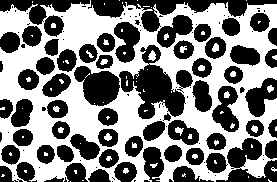
\includegraphics[width=6.3cm]{redblood.png}
    \caption{Original image, (277\times182)}
    \label{fig:erosionSym}
\end{figure}

\begin{flushleft}
In order to assist in the counting of the red blood cells present in this image, we would first remove the evident noise then proceed to fill in the holes in the middle of the cells as best as possible. 
\end{flushleft}
\begin{figure}[ht] 
  \label{ fig7} 
  \begin{minipage}[b]{0.5\linewidth}
    \centering
    \includegraphics[width=.97\linewidth]{c_redbloodse4.png} 
    \caption{Closing with SE4} 
    \vspace{4ex}
  \end{minipage}%%
  \begin{minipage}[b]{0.5\linewidth}
    \centering
    \includegraphics[width=.97\linewidth]{e_closedredbloodse3.png} 
    \caption{Erosion of Fig.13 (SE3)} 
    \vspace{4ex}
  \end{minipage} 
\end{figure} 

\begin{flushleft}
We decided to perform a closing operation to remove the small black spots present then fill in some of the white spaces present in the cell. After comparing the results of a size 3 and size 4 square, we found that the latter worked better in removing the noisy elements within this picture. \newline
Performing the closing led to the red blood cells not being as defined. In order to fill in the holes and accentuate the features of the cells we decided to perform a erosion on the closed image using a vertical SE of length 3. \newline
However, additional operations would need to be done in order to further fill in the center of some of the cells. 
\end{flushleft}

\subsection{Fingerprint image cleaning}
\begin{flushleft}
In this experiment we try to remove some of the noise present in this fingerprint image (Figure 15) and sharpen the image further to create a clearer result. There is a bit of noise surrounding the fingerprint so we decided to use a square of size 3 (SE1.txt) in order to remove this noise. After performing an erosion we get an image without the white squares (Figure 16), however it also leads to a darker fingerprint. In order to further define the print lines we decided to perform an erosion which produces a far better result (Figure 17) leave us with a clear and defined fingerprint.
\end{flushleft}
\begin{figure}[H]
    \centering
    \includegraphics[height=8cm]{fingerprint.png}
    \caption{Original image, (332\times450)}
    \label{fig:erosionSym}
\end{figure}
\begin{figure}[H] 
  \label{ fig7} 
  \begin{minipage}[b]{0.5\linewidth}
    \centering
    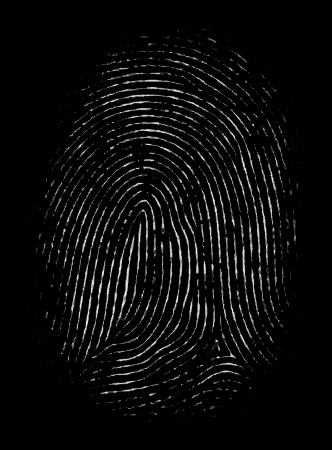
\includegraphics[height=.97\linewidth]{e_fingerprint.png} 
    \caption{Closing with SE4} 
    \vspace{4ex}
  \end{minipage}%%
  \begin{minipage}[b]{0.5\linewidth}
    \centering
    \includegraphics[height=.97\linewidth]{o_fingerprint.png} 
    \caption{Erosion of Fig.16 (SE3)} 
    \vspace{4ex}
  \end{minipage} 
\end{figure} 
\begin{flushleft}
\end{flushleft}

\newpage

\section{Comparison}
\begin{flushleft}
After writing down the algorithms their time complexities we figured these operations are slow to compute in practice especially for large structuring elements. We then decided to compared our implementation to the OpenCV erode and dilate functions and found that on average our implementation processes a 512x512 image with a structuring element of size 3x3 in $2.4344s$ while the OpenCV function preforms it in $0.0001242s$ which made us realize there must be plenty of more efficient approaches. 
\end{flushleft}

\section{Task Distribution}
\begin{flushleft}
Regarding the task distribution, we decided to split up the work evenly. These were our tasks. \newline
Otmane Sabir : \newline
\begin{enumerate}
    \item Wrote function for finding minimum and wrote erosion
    \item Wrote function for opening
    \item Ran test 1-7 and ran the fingerprint and cell tests
    \item Wrote 2 chapters of the report.
\end{enumerate}
Aadil Anil Kumar : \newline
\begin{enumerate}
    \item Wrote function for finding maximum and wrote dilation
    \item Wrote function for dilation
    \item Ran the rest of the test and 3 experiments
    \item Wrote 2 chapters of the report.
\end{enumerate}
\end{flushleft}

\begin{thebibliography}{}
\bibitem{Wikipedia} 
Erosion (morphology),
\\\texttt{https://en.wikipedia.org/wiki/Erosion_(morphology)}

\bibitem{Wikipedia} 
Dilation (morphology),
\\\texttt{https://en.wikipedia.org/wiki/Dilation_(morphology)}

\bibitem{MathWorks} 
Types of Morphological Operations,
\\\texttt{https://www.mathworks.com/help/images/morphological-dilation-and-erosion.html}

\bibitem{HIRP2} 
Morphology,
\\\texttt{https://homepages.inf.ed.ac.uk/rbf/HIPR2/morops.htm}

\bibitem{OpenCV2} 
Eroding and dilating,
\\\texttt{https://docs.opencv.org/2.4/doc/tutorials/imgproc/erosion_dilatation/erosion_dilatation.html}

\bibitem{Book} 
Nick Efford. 
\textit{Digital Image Processing: A Practical Introduction Using Java} 
Pearson Education, 2000.

\end{thebibliography}
\end{document}
